\section{The master equation of direct detection}\label{sec:1.1}

A dark-matter detector counts events. Each one is a small burst of electron--hole pairs, phonons, quasiparticles or photons, released when a particle from the Galactic halo gives up an energy $\omega$ and a momentum $\vect{q}$ to the target. Theory has to predict the number of events that a kilogram of target collects per year, the \emph{event rate} $\mathcal{R}$, and the distribution of these events in $\omega$. Take dark matter $\chi$ of mass $\mchi$ that scatters on the electrons of the target, through an interaction that couples to the electron density and not to the electron spins. The event rate then has the form
\begin{equation}
  \mathcal{R} = \frac{1}{\rho_T}\,\underbrace{\frac{\rho_\chi}{\mchi}\int\dd^3v\,f_\chi(\vect{v})}_{\text{halo}}\int\frac{\dd^3q}{(2\pi)^3}\,\underbrace{|\tilde V(\vect{q})|^2}_{\text{coupling}}\int\dd\omega\,\underbrace{S(\vect{q},\omega)}_{\text{target}}\,\underbrace{\delta\!\left(\omega - \vect{q}\cdot\vect{v} + \frac{q^2}{2\mchi}\right)}_{\text{kinematics}}.
  \label{eq:1.1-rate}
\end{equation}
We will derive it in the chapters that follow: \cref{chap:2} obtains it from Fermi's golden rule (\cref{eq:2.5-golden}), and once the directions of $\vect{q}$ are averaged it reduces to \cref{eq:1.5-rate}, the form used for limits~\cite{kahn2022searches}.

The integrand is the product of the halo, the coupling and the response of the target, joined by a delta function. The halo enters through $\rho_\chi/\mchi$, the number density of dark-matter particles near the Earth, with $\rho_\chi$ their mass density, and through $f_\chi(\vect{v})$, the distribution of their velocities $\vect{v}$ in the laboratory, normalized to one. The coupling is $\tilde V(\vect{q})$, the Fourier transform of the potential between a dark-matter particle and an electron, and $|\tilde V(\vect{q})|^2$ weights each momentum transfer by the strength of the dark-matter--electron interaction at that momentum. The response is the \emph{dynamic structure factor} $S(\vect{q},\omega)$ of the electron density. The dynamic structure factor measures how readily the solid absorbs a momentum $\vect{q}$ together with an energy $\omega$. At zero temperature it is a sum over the excited states of the solid that lie an energy $\omega$ above its ground state. Each term is the squared matrix element of the electron density at wavevector $\vect{q}$ between the ground state and the excited state. A factor $2\pi$ comes from the golden rule, and a division by the volume of the target makes $S$ independent of the size of the target (\cref{eq:2.5-golden}; \cref{sec:4.2}). The delta function is energy conservation. A particle whose momentum changes by $\vect{q}$ loses the kinetic energy $\vect{q}\cdot\vect{v} - q^2/2\mchi$, and the target must take up exactly that amount. Finally, $1/\rho_T$, with $\rho_T$ the mass density of the target, turns a rate per unit volume into a rate per unit target mass, the unit in which experiments quote event rates.

Each factor of \cref{eq:1.1-rate} belongs to a different body of physics. The halo is astrophysics, the coupling is particle physics, and the response is condensed-matter physics; only the kinematics of the delta function connects them, and it involves only $\vect{q}$, $\vect{v}$, $\omega$ and $\mchi$. As a result, a new dark-matter model changes $|\tilde V|^2$ and leaves $S$ alone, while a new target changes $S$ and leaves the coupling alone. A response computed once for silicon serves every model that couples to the electron density, and once $S$ is tabulated, a limit can be recast for another model by weighting $S$ with the new coupling, without computing the response of the solid again. The response involves of order $10^{23}$ interacting electrons per cubic centimeter in a periodic lattice, and computing it is most of what this book does.

The halo needs no new physics. Its local density and velocity distribution are adopted from astronomy by convention: $\rho_\chi = \SI{0.3}{GeV.cm^{-3}}$ and a Maxwellian with speeds near $10^{-3}$ in units of the speed of light, seen from a laboratory that moves through the halo (\cref{sec:1.2}). Since the delta function involves no property of the target, much of what a detector can reach follows before any target is specified (\cref{sec:1.3}). Kinematics fixes the smallest speed $\vmin$ that can deposit a given $\omega$ at a given $q$, and it fixes the lightest mass that can get over a detector threshold. Once the velocity integral is done, the halo enters only through $\eta(\vmin)$, the mean inverse speed above $\vmin$. The coupling is a choice of model. Its simplest form is the exchange of a \emph{mediator}, a particle that carries the interaction between the dark matter and the electron. The coupling then condenses into $|\tilde V(q)|^2 = \pi\sigmae\FDM(q)^2/\mu_{\chi e}^2$ (\cref{eq:1.4-Vsq}), with the reduced mass $\mu_{\chi e}$ of the dark matter and the electron, a reference cross-section $\sigmae$ that sets the strength, and a form factor $\FDM(q)$ that carries the momentum dependence (\cref{sec:1.4}). An experiment then quotes its result as a limit on $\sigmae$ at each mass. The response, however, is a many-body problem. It needs the electronic states of a crystal, the linear response of its electrons, the vibrations of its lattice and the electron--phonon coupling (\cref{chap:3,chap:4,chap:5,chap:6,chap:7}). The response also needs a framework that holds for any coupling (\cref{chap:8}) and a separate treatment of each excitation channel. Even an exact $S$ does not finish the calculation, because a detector does not record $\omega$. It records the charges, phonons, quasiparticles or photons into which the deposited energy relaxes, and the conversion of the deposited energy into these quanta is the last link between the event rate and a measured count (\cref{sec:1.5}).

The product in \cref{eq:1.1-rate} is the simplest case, one coupling to one density, and the book generalizes it in several directions without losing the separation of the three factors. Dark matter can couple to more than the electron density, to nuclei, spins or currents as well, and the single $S$ then becomes a matrix of response functions, with one entry for each pair of couplings. The off-diagonal entries of this matrix make the contributions of different couplings interfere (\cref{chap:8}). The electrons of the target also rearrange to screen the dark-matter potential. For a mediator that mixes with the photon, the screened response that takes the place of $S$ is the \emph{loss function}, the imaginary part of the inverse dielectric function (\cref{sec:10.2}). A bosonic dark-matter particle can instead be absorbed. It deposits its whole mass $m_\phi$ at almost zero momentum, and the absorption rate is then set by the optical conductivity of the target at $\omega = m_\phi$ instead of by a scattering response (\cref{sec:1.4}). Other processes need more than one response at once. In the Migdal effect a recoiling nucleus shakes off an electron, so the Migdal rate takes the joint response of electrons and lattice (\cref{chap:12}). At an indirect gap the highest filled and the lowest empty electron states differ in crystal momentum (\cref{sec:1.3}). An electron excited across an indirect gap needs a phonon to supply this difference in crystal momentum, and the excitation is then a second-order process (\cref{chap:13}). Finally, no computed response is exact. Each $S$ in the book names the approximation behind it and comes with an estimate of its error, and \cref{chap:21} carries those errors into the exclusion limits.

\subsection{Inputs from cosmology}

All of the evidence for dark matter is gravitational. Stars and gas in spiral galaxies orbit at a circular speed $v_{\mathrm{c}}$ that stays flat far outside the luminous disk, where the visible mass alone would make $v_{\mathrm{c}}$ fall as $r^{-1/2}$ with the galactocentric radius $r$. A flat rotation curve needs an enclosed mass that grows linearly with $r$ where almost no light is emitted~\cite{rubin1980rotational,bertone2018history}. The anisotropies of the cosmic microwave background (CMB) fix the total amount of dark matter, because dark matter does not take part in the acoustic oscillations of the photon--baryon plasma before recombination, and its potential wells shape the relative heights of the acoustic peaks~\cite{aghanim2020planck}.

None of this gravitational evidence identifies the dark-matter particle. The observations measure a mass density, and for detection they supply two numbers. The local density $\rho_\chi$ comes from the motion of stars near the Sun and from the rotation curve of the Milky Way~\cite[Sect.~3.1]{green2012astrophysical}; \cref{sec:1.2} gives the measured range and the value we use. The cosmological abundance is quoted as $\Omega_{\mathrm{c}}h^2$, where $\Omega_{\mathrm{c}}$ is the mean density of cold dark matter as a fraction of the critical density (the density of a spatially flat universe), and $h$ is the present Hubble rate in units of \SI{100}{km.s^{-1}.Mpc^{-1}}. The CMB anisotropies, with CMB lensing, give~\cite[Table~2 and Eq.~(23)]{aghanim2020planck}
\begin{equation*}
  \Omega_{\mathrm{c}} h^2 = \num{0.1200(12)},
\end{equation*}
usually quoted as $0.120 \pm 0.001$. The baryon density from the same fit, \num[group-digits=none]{0.02237(15)} in the same units, is smaller than $\Omega_{\mathrm{c}}h^2$ by a factor of 5.4.

Gravity cannot fix the mass $\mchi$ of the dark-matter particle: by the equivalence principle, a test body falls the same way whatever its mass, and every observation above measures the mass density $\nd_\chi\mchi$ alone, with $\nd_\chi$ the number density. The mass enters only where the particle picture itself fails. At the light end, a boson with $\mchi \approx \SI{e-22}{eV}$ has a de~Broglie wavelength comparable to the size of a dwarf galaxy, and lighter fields cannot cluster on that scale. Fermions need $\mchi$ above a few hundred eV so that halo phase-space densities stay below the Pauli limit, the largest density that the exclusion principle allows; the argument is related to the Tremaine--Gunn bound~\cite{tremaine1979dynamical,lin2019tasi}. A particle once in equilibrium with the plasma must be heavier than roughly a keV, or it moves fast enough to erase observed small-scale structure~\cite[Sect.~I\,A]{lin2019tasi}. At the heavy end, fundamental particles reach the Planck mass, and compact objects such as primordial black holes extend to tens of solar masses~\cite[Sect.~I\,C]{lin2019tasi}. The allowed range spans about 90 decades (\cref{fig:1-massrange}).

\begin{figure}[tbp]
  \centering
  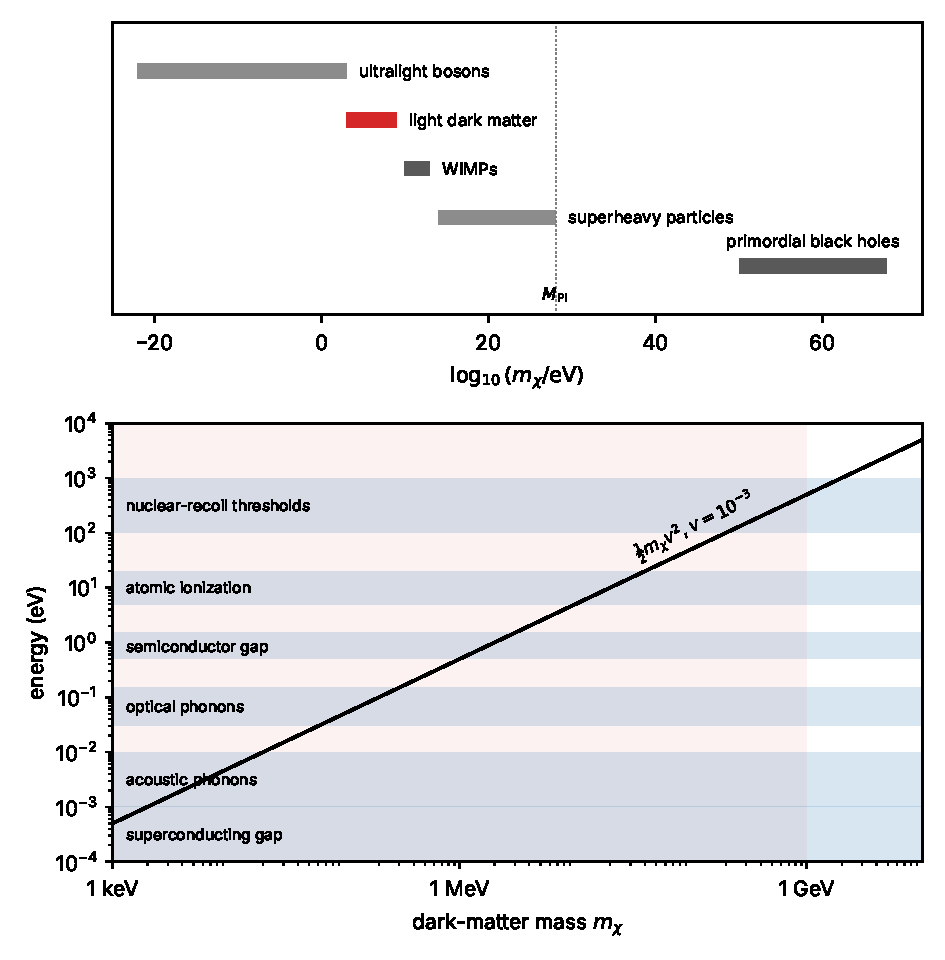
\includegraphics[width=\linewidth]{figures/ch01/fig1_1.pdf}
  \caption{Top: masses of dark-matter candidates, from ultralight bosonic fields to primordial black holes; the dotted line marks the Planck mass. Ranges follow Ref.~\cite[Sect.~I]{lin2019tasi}. Bottom: the keV--GeV window (shaded red). The solid line is the kinetic energy $\frac12 m_\chi v^2$ of dark matter moving at $v = 10^{-3}$. The blue bands are the energy scales of excitations in solids and the thresholds of nuclear-recoil detectors~\cite{kahn2022searches}.}
  \label{fig:1-massrange}
\end{figure}

Within this range, the window between a keV and a GeV has been tested least. Dark matter bound to the Galaxy moves at $v \approx 10^{-3}$, so its kinetic energy $\frac12 \mchi v^2$ is \SI{0.5}{keV} for \SI{1}{GeV}, \SI{0.5}{eV} for \SI{1}{MeV} and \SI{0.5}{meV} for \SI{1}{keV}. A \SI{1}{GeV} particle can deposit at most about \SI{0.1}{keV} in a xenon nucleus (\cref{sec:1.3}). A deposit of \SI{0.1}{keV} is below the thresholds of ton-scale xenon detectors, which read the scintillation and ionization of the recoiling nucleus: Ref.~\cite[Sect.~I]{kahn2022searches} places these thresholds at the few-hundred-eV scale, and the thresholds of analyses that require both signals lie nearer a keV. Solids, however, have excitations across the range of these kinetic energies: typical electronic band gaps of an eV and optical phonons of tens of meV~\cite[Table~I]{kahn2022searches}, and acoustic phonons and superconducting gaps at the meV scale and below (\cref{sec:1.3,sec:1.5}). Particles in this window, between a keV and a GeV, are what the field calls \emph{light dark matter}, or sub-GeV dark matter.
